\chapter{Metodologia}

A metodologia do presente trabalho é dividida em três principais partes. A primeira é a etapa de projeto dos componentes mecânicos que fazem parte do satélite, entre eles: as rodas de reação, motor DC (Direct Current - corrente contínua), mancal a ar e hastes. Também contempla as especificação dos componentes eletrônicos que constituem o satélite. É na segunda etapa que ocorre a modelagem completa do sistema e especificações das limitações de movimentação do satélite, juntamente com a elaboração dos diagramas de blocos do controle. Nessa etapa também é feita a modelagem do motor DC, para que possa fornecer torque para romper a inércia da planta. Já na terceira etapa, são abordados os elementos de software, de rede e supervisão do satélite. Nessa etapa também se encontram as especificações de software, desenvolvimento do software de controle e supervisão.


%%%%%%%%%%%%%%%%%%%%%%%%%%%%%%%%%%%%%%%%%%%%%%%%%%%%%%%%%%%%%%%%%%%%%%

\section{Hardware}

Após a modelagem descrita no referencial teórico, é possível modelar um simulador de satélite de fabricação factível.  O mancal a ar, a base de suporte do simulador do satélite, rodas de reação, motores Brushless (motor de corrente contínua sem escovas) e os outros elementos, podem ser vistos na figura \ref{fig:satelite_completo}.

\begin{figure}[H]
  \caption{Desenho Mecânico Completo do Simulador de Satélite}
  \begin{center}
      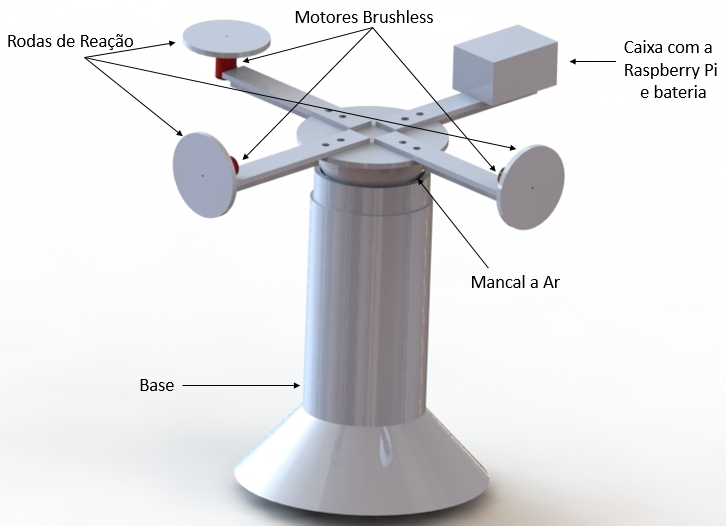
\includegraphics[scale=.5]{metodologia/img/satelite_completo}
  \end{center}
  \fonte{Elaborado pelo Autor.} 
  \label{fig:satelite_completo}
\end{figure}

 Como podemos ver na imagem anterior, o modelo sofre várias simplificações em relação a um satélite real, onde o modelo passa a ser de fácil implementação, possibilitando a validação dos conceitos propostos nesse trabalho. Dentre várias simplificações, a mais óbvia, o simulador não apresentará de forma direta os movimentos de translação descritos no seção \ref{cap:dinamica}. Ainda, existe uma limitação para os ângulos $\phi$, $\theta$ e $\psi$ que é um intervalo de $0<\phi, \theta, \psi<240º$ devido a existência do mancal a ar e a simetria do corpo do satélite, como princípio para simplificar a modelagem matemática do mesmo. Os principais elementos do simulador de satélites, serão descritos de forma detalhada na sequência, dentre eles, o corpo do satélite.


%%%%%%%%%%%%%%%%%%%%%%%%%%%%%%%%%%%

\subsection{Corpo do Simulador de Satélite}

O elemento de dinâmica mais importante que deve ser dimensionado, é o corpo do satélite. É nele que são fixados todos os outros elementos que compõem o simulador de satélites. Para isso, optamos como material, o alumínio, pois possui menor densidade e resistência mecânica adequada ao projeto. Na figura abaixo podemos ver o corpo do simulador.

\begin{figure}[H]
  \caption{Corpo do Simulador de Satélites}
  \begin{center}
      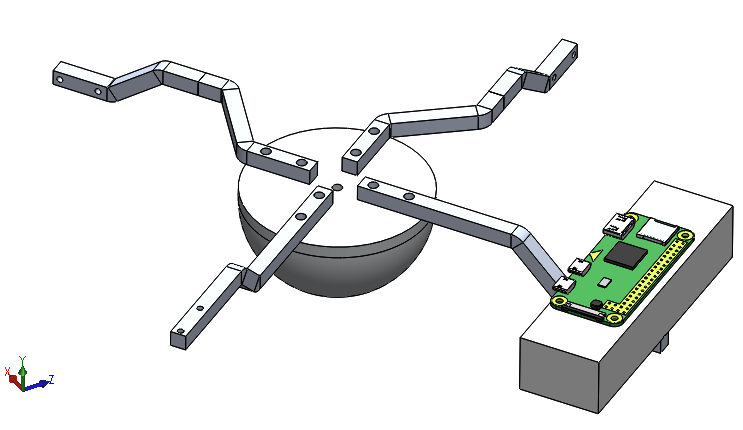
\includegraphics[scale=.4]{metodologia/img/corpo_satelite}
  \end{center}
  \fonte{Elaborado pelo Autor.} 
  \label{fig:corpo_satelite}
\end{figure}


Onde \textit{hx} é a haste do motor que atua no eixo x, \textit{hy} é a haste do motor que atua no eixo y, \textit{hz} é a haste do motor que atua no eixo z, \textit{hb} é a haste da bateria e \textit{se} é a semiesfera que é a interface entre o corpo e o mancal a ar. Esse último será explicado na sequência. O projeto leva em consideração a distribuição de massa e os centros de massa, pois o simulador de satélite deve ficar o mais simétrico e em equilíbrio possível, facilitando a atuação do controle que prevê sua simetria.

Através do software de desenho mecânico, SolidWorks, onde o projeto foi desenvolvido, conseguimos calcular o peso do satélite, que é de aproximadamente $\SI{1.25}{\kg}$, contado com a bateria de polímero de Lítio e outro periféricos. Esse valor é necessário para o dimensionamento das rodas de reação, que também será descrito na sequência. Ainda, com o mesmo software, conseguimos os valores de momento de inércia máximo entre os eixos que é de aproximadamente $\SI{0.5}{\kg\meter\squared}$, o qual é usado para dimensionamento das rodas de reação


%%%%%%%%%%%%%%%%%%%%%%%%%%%%%%%%%%%

\subsection{Mancal a Ar}

Um dos elementos mais importantes do simulador, é o mancal a ar. Ele possibilita a criação mínima de atrito entre a esfera e a região côncava, pois existe um fluxo de ar promovido por um sistema pneumático que cria uma camada de ar entre as duas partes. Com isso, a esfera fica com movimento praticamente livre de atritos dentro de uma região limitada pela geometria da esfera, o corpo do satélite, a massa do satélite e a pressão do sistema pneumático. O modelo mecânico do mancal com seus elementos podem ser vistos na figura \ref{fig:base_desenho}.

\begin{figure}[H]
  \caption{Desenho Mecânico do Mancal a Ar}
  \begin{center}
      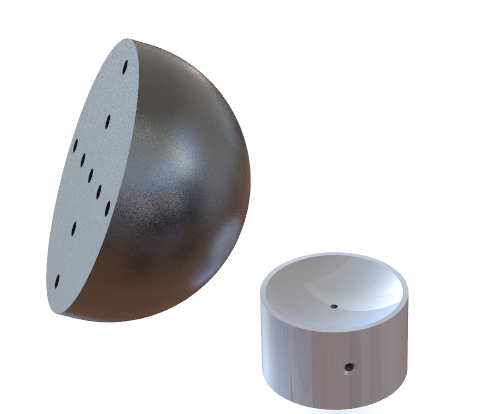
\includegraphics[scale=.45]{metodologia/img/base_desenho}
  \end{center}
  \fonte{Elaborado pelo Autor.} 
  \label{fig:base_desenho}
\end{figure}

O mancal precisou ser usinado, deviso a precisão do encaixe entre a esfera e a região concava, para que a camada de ar seja o mais homogênea possível, evitando turbulências e regiões com atrito maiores que em outras. 


%%%%%%%%%%%%%%%%%%%%%%%%%%%%%%%%%%%

\subsection{Motor CC e Rodas de Reação}

Como foi descrito no referencial, os atuadores do satélite serão rodas de reação acopladas em motores de corrente contínua (CC). Na sequência, são descritos os cálculos das rodas de reação e a escolha dos motores CC. 


\subsubsection{Projeto das Rodas de Reação}

Partindo do princípio da conservação do momento angular do corpo do satélite, precisamos dimensionar o momento angular da roda e, por consequência, os momentos de inércia delas. Para isso, precisamos calcular o momento angular do satélite, que pode ser descrito como:

\begin{equation}
\vec{L_{sat}} = 2\left(I_{sat} + m\left(\frac{r_{sat}}{2}\right)^2\right)  
\end{equation}

Cada roda será responsável por um terço do momento angular total do satélite, como pode ser visto na sequência:

\begin{equation}
\vec{L_{roda}} = \frac{\vec{L_{sat}}}{3}   
\end{equation}

Onde $I_{sat}$ é o momento de inércia do satélite, $m$ é a massa, $r_{sat}$ é a distância dos motores do centro de inércia. Podemos relacionar o momento angular com o momento de inércia das rodas e a velocidade angular, como podemos ver abaixo.

\begin{equation}
\vec{L_{roda}} = I_{roda}\vec{\omega_{roda}}
\end{equation}

Conseguimos dimensionar o momento angular das rodas através da variação do momento de inércia ou rotação das rodas. Com o objetivo de controlar o satélite, varia-se a velocidade angular das rodas com momento de inércia fixo. Na figura \ref{fig:motor_roda_desenho2}, temos o desenho escolhido para o projeto das rodas, pois concentramos mais massa na extremidade, contribuindo assim, para um maior momento de inércia.

\begin{figure}[H]
  \caption{Geometria Básica para o Projeto de Rodas de Reação}
  \begin{center}
      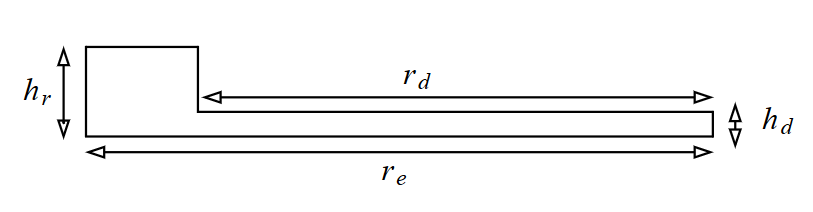
\includegraphics[scale=.45]{metodologia/img/roda_reacao_modelo}
  \end{center}
  \fonte{Elaborado pelo Autor.} 
  \label{fig:motor_roda_desenho2}
\end{figure}

Essa geometria escolhida, possui momento de inércia que pode ser descrito pela seguinte equação:

\begin{equation}
\vec{I_{roda}} = \rho \frac{\pi}{2}(h_r(r_{e}^4-r_d^4)+h_dr_d^4) 
\end{equation}

Onde $\vec{I_{roda}}$ é o momento de inércia da roda, $\rho$ é a densidade do material que compõe a roda, $h_r$ é a espessura da borda, $h_d$ é a espessura do disco, $r_e$ é o raio total da roda e $r_d$ é o raio do disco. Um conjunto de parâmetros que satisfazem as equações a cima descritas à uma velocidade angular de $\SI{230.38}{\radian\per\second}$(2200 RPM), são: 

\begin{table}
  \caption{Dimensões das Rodas de Reação}
  \label{tab:bias_correction}
  \centering%
  \begin{minipage}{.42\textwidth}
    \begin{tabular*}{\textwidth}{cc}
      \hline
      {Dimensão} & Unidade \\ \hline
      \hline
      $\rho$  &  $\SI{7860}{\kilogram\per\cubic\metre}$ (Aço SAE 1045)\\ 
      $h_r$   &  $\SI{10.5}{\milli\metre}$ \\
      $h_d$   &  $\SI{2}{\milli\metre}$  \\
      $r_e$   &  $\SI{37}{\milli\metre}$  \\
      $r_d$   &  $\SI{30}{\milli\metre}$  \\ \hline
    \end{tabular*}
    \fonte{Elaborado pelo Autor.} 
  \end{minipage}
\end{table}


%%%%%%%%%%%%%%%%%%%%%%%%%%%%%%%%%%%

\subsubsection{Escolha dos Motores CC}

O atuador do simulador de satélite será um conjunto de três motores Brushless dispostos um em cada eixo cartesiano. Juntamente com esses motores, são acopladas rodas de reação, que juntamente com os motores, farão os movimentos de rotação do satélite. Como vimos na imagem \ref{fig:satelite_completo}, os motores e as hastes estão distribuídos de forma simétrica e afastados do centro de massa do satélite, para facilitar a movimentação promovida pelo torque dos motores. O modelo de motor escolhido foi o \textit{Turnigy D2826-6 2200kV}, que é um motor usado em aeromodelos e possui um empuxo de aproximadamente $\SI{960}{\milli\gram}$ e relação de velocidade por Volt de 2200 RPM por Volt. Na imagem \ref{fig:motor_roda_desenho} podemos ver parte da haste, o motor e a roda de reação acoplados. 

\begin{figure}[H]
  \caption{Desenho mecânico do conjunto Motor-Roda}
  \begin{center}
      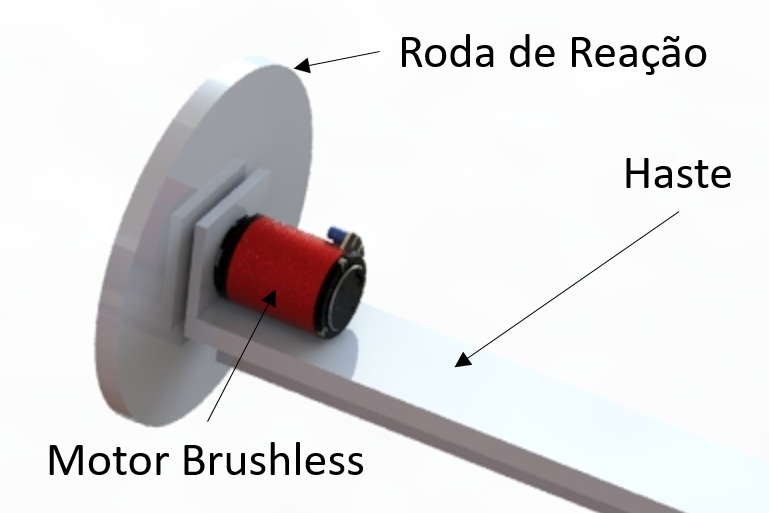
\includegraphics[scale=.45]{metodologia/img/motor_roda_desenho}
  \end{center}
  \fonte{Elaborado pelo Autor.} 
  \label{fig:motor_roda_desenho}
\end{figure}

A roda de reação também foi usinada, pois é necessário uma roda com uma massa e formato específico, para que possa ser acoplar ao motor e o conjunto consiga realizar os movimentos propostos. 


%%%%%%%%%%%%%%%%%%%%%%%%%%%%%%%%%%%

\subsection{Elementos Eletrônicos}

A placa de desenvolvimento e prototipação de sistemas embarcados Raspberry Pi Zero W (RPi) foi a escolhida, pois ela conta com os elementos mínimos de interfaceamento com os atuadores e outros periféricos. Além disso, ela possui conectividade wireless (sem fio), possibilitando a supervisão e controle do satélite sem fio. Como o trabalho terá o seu desenvolvimento baseado em desenvolvimento de software e adaptações do sistema operacional, uma placa com suporte, boa documentação e comunidade ativa, facilita o desenvolvimento. Uma representação dessa placa pode ser vista na figura \ref{fig:rasp_zero}

\begin{figure}[H]
  \caption{Raspberry Pi Zero W}
  \begin{center}
      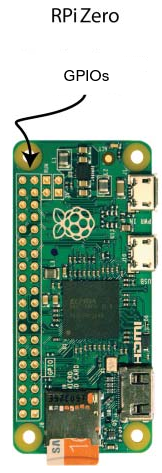
\includegraphics[scale=.55]{metodologia/img/rasp_zero}
  \end{center}
  \fonte{Adaptado de \citeonline{Molloy2016}} 
  \label{fig:rasp_zero}
\end{figure}

Um outro elemento que será indispensável é o acelerômetro, o qual será o sensor de realimentação da posições angulares do satélite. Sua comunicação com a RPi será através da interface I2C, que será descrita na seção de software. O acelerômetro informará o modelo da posição angular em graus, através da integral da velocidade instantânea em cada eixo.

\begin{figure}[H]
  \caption{Placa de Circuito impresso com o acelerômetro e Giroscópio MPU6050}
  \begin{center}
      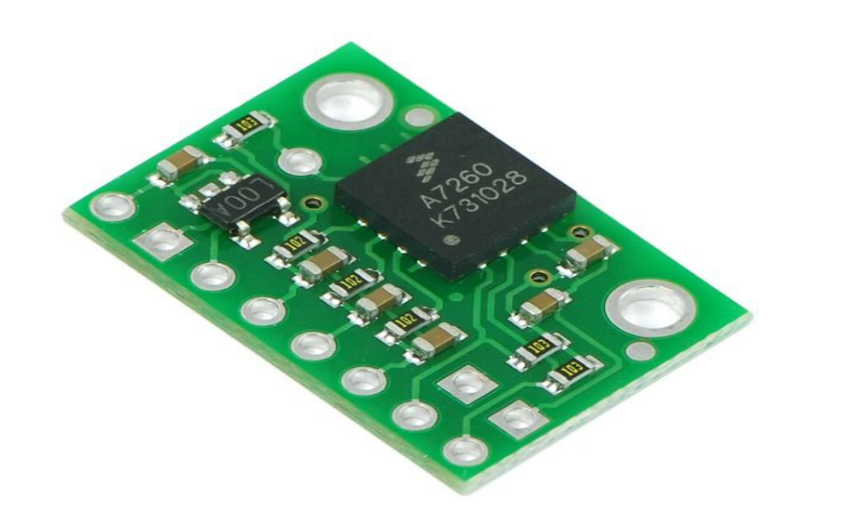
\includegraphics[scale=.4]{metodologia/img/pci_acelerometro_calache_p22}
  \end{center}
  \fonte{Adaptado de \citeonline{mpu}} 
  \label{fig:pci_acelerometro_calache_p22}
\end{figure}

Ainda, para o acionamento dos motores Brushless serão utilizados ESC (Electronic-Speed-Control - Controlador eletrônico de velocidade) que serão conectados com a bateria, os motores e a RPi. Após a conclusão do dimensionamento e escolha dos materiais, foi possível fazer a fabricação mecânica e montagem do simulador satélite, o qual pode ser visto nas figuras \ref{fig:base_real}, \ref{fig:corpo_real} e \ref{fig:simulador_real}.

\begin{figure}[H]
  \caption{Base do Simulador de Satélites Prototipado}
  \begin{center}
      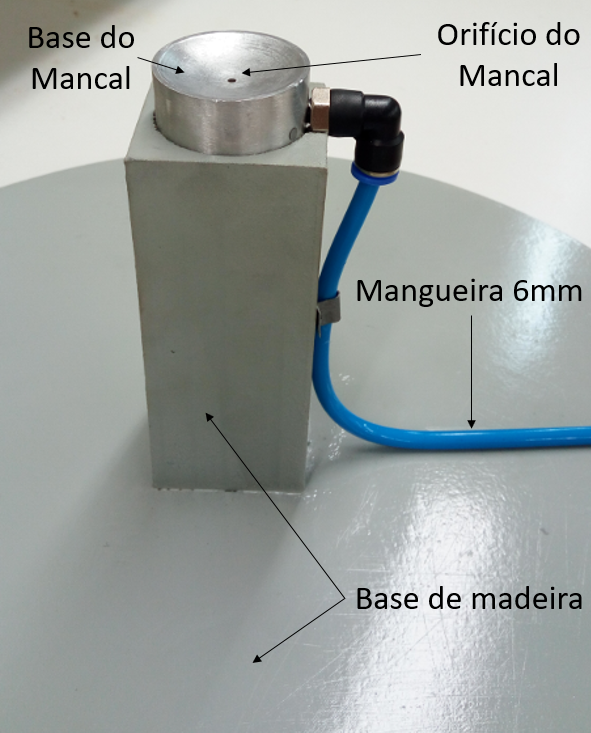
\includegraphics[scale=.5]{metodologia/img/base_real}
  \end{center}
  \fonte{Elaborado pelo Autor.} 
  \label{fig:base_real}
\end{figure}

Na imagem anterior, podemos ver a base do simulador, feita em madeira, onde se encontra a região concava do mancal e as conexão 
pneumáticas. Já na figura \ref{fig:corpo_real}, podemos ver as partes que compõem o corpo do simulador.

\begin{figure}[H]
  \caption{Simulador de Satélites Prototipado}
  \begin{center}
      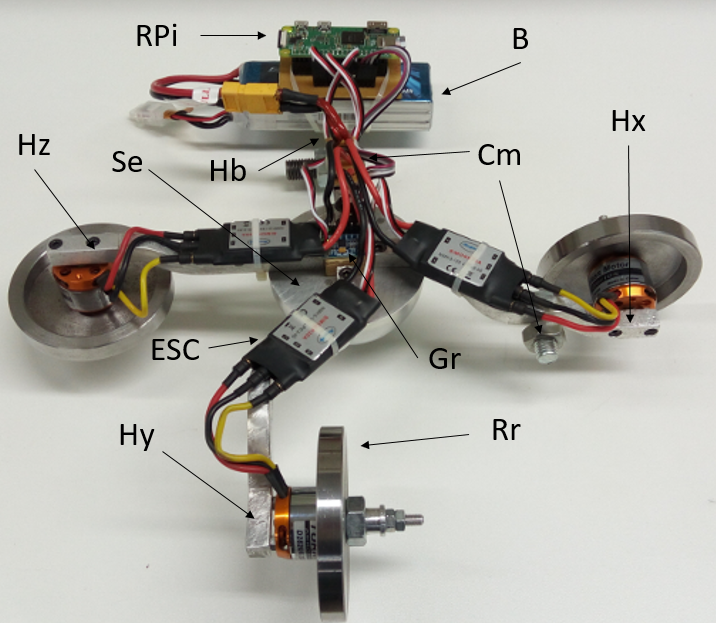
\includegraphics[scale=.65]{metodologia/img/corpo_real}
  \end{center}
  \fonte{Elaborado pelo Autor.} 
  \label{fig:corpo_real}
\end{figure}

Onde \textit{Rpi} é a Rapberri Pi Zero W, \textit{B} é bateria, \textit{ESC} são os controladores, \textit{Rr} são as rodas de reação, \textit{Cm} são massas para compensação de massa do simulador, \textit{Gr} é o acelerômetro/giroscópio, \textit{Se} é a semiesfera de alumínio que compõe o mancal, \textit{Hb} é a haste de alumínio da bateria, \textit{Hx} é a haste do motor do eixo x, , \textit{Hy} é a haste do motor do eixo y e \textit{Hz} é a haste do motor do eixo z. E por fim, a imagem completa do simulador de satélites, que pode ser vista na figura \ref{fig:simulador_real}.

\begin{figure}[H]
  \caption{Simulador de Satélites Prototipado}
  \begin{center}
      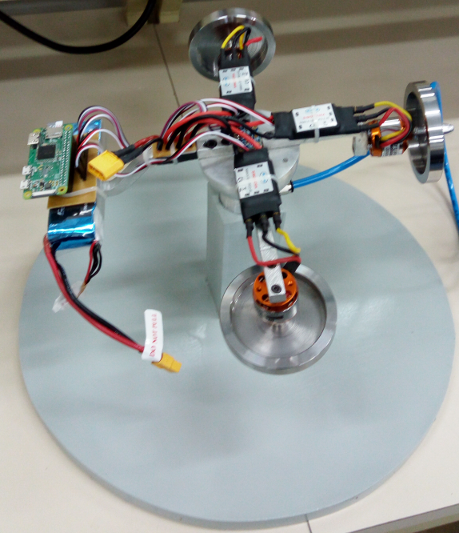
\includegraphics[scale=.65]{metodologia/img/simulador_real}
  \end{center}
  \fonte{Elaborado pelo Autor.} 
  \label{fig:simulador_real}
\end{figure}

Com isso, todos os principais elementos de hardware foram descritos, sendo a modelagem dos mesmos o próximo passo do desenvolvimento.


%%%%%%%%%%%%%%%%%%%%%%%%%%%%%%%%%%%%%%%%%%%%%%%%%%%%%%%%%%%%%%%%%%%%%%

\section{Sistemas de Controle}

Após a descrição dos conceitos básicos de controle e do modelo mecânico do satélite, é possível desenvolver os modelos da planta e do sistema de controle. Ainda nessa seção, será descrita a modelagem do motor de corrente contínua sugerido na seção anterior e posteriormente a modelagem completa do simulador de satélites.


%%%%%%%%%%%%%%%%%%%%%%%%%%%%%%%%%%%
\subsection{Modelo Motor DC}

Após a escolha do tipo de motor que será utilizado como atuador no controle da atitude do satélite, se faz necessário a modelagem do mesmo, para que consigamos acoplar ao modelo do satélite, o torque que promoverá a variação mo momento angular do satélite, e por consequência, a posição angular. A figura \ref{fig:modelo_motor_dc} representa o modelo elétrico associado ao momento de inércia do rotor $J_{\omega 1}$ ao rotor e a da roda de reação $J_{\omega 2}$

\begin{figure}[H]
  \caption{Modelo do Motor DC}
  \begin{center}
      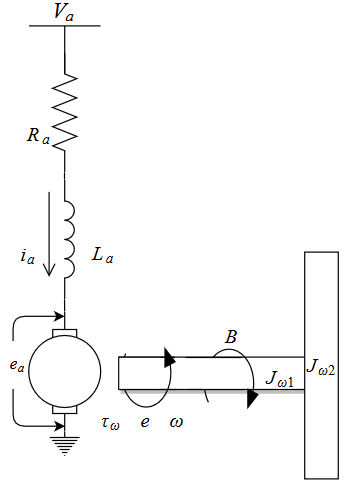
\includegraphics[scale=.7]{metodologia/img/modelo_motor_dc}
  \end{center}
  \fonte{Elaborado pelo Autor.} 
  \label{fig:modelo_motor_dc}
\end{figure}

Onde $R_a$, $L_a$, $i_a$ e $e_a$ são a resistência, a indutância, a corrente e a tensão de armadura, respectivamente, $e_b$ é a tensão induzida e $\tau_{\omega}$ é o torque do motor. A relação entre a corrente com a tensão de armadura pode ser vista na sequência \cite{Ogata}.

\begin{equation}
L_a \frac{di_a}{dt}+R_a i_a + e_b = e_a
\end{equation}

Como existe a relação entre a constante de torque $K_t$ e a tensão induzida, juntamente com a relação entre a constante de velocidade contra-eletromotriz $K_w$ e a tensão da fonte $V_a$. Isso pode ser visto na sequência.

\begin{equation}
  e_a = K_t\frac{d\theta}{dt}
\end{equation}

e

\begin{equation}
  e_b = K_wV_a
\end{equation}

Temos que:

\begin{equation}\label{eq:la}
L_a \frac{di_a}{dt}+R_a i_a + K_t\frac{d\theta}{dt} = K_wV_a
\end{equation}

Ainda, a relação que através do conceito de equilíbrio de torque, conseguimos relacionar o torque do motor $\tau_{\omega}$ com os momentos de inércia do rotor e da roda de reação com a corrente da armadura da seguinte forma:

\begin{equation}\label{eq:tauj}
\tau_{\omega} = (J_{\omega 1} + J_{\omega 2})\frac{d^{2}\theta}{dt^{2}}+B\frac{d\theta}{dt} = K_t i_a
\end{equation}

Onde B é o atrito viscoso. Como queremos relacionar a tensão da fonte com a velocidade angular, devemos manipular as equações \ref{eq:la} e \ref{eq:tauj} e aplicarmos a transformada de Laplace. O resultado dessas operações pode ser visto na sequência: 

\begin{equation}
  \frac{\omega(s)}{V_a(s)} = \frac{K_wK_t}{(R_a+ sLa)(s(J_{\omega 1} + J_{\omega 2})+B)+K_wK_t}  
\end{equation}

Mas como nas equações \ref{eq:modeloA}, \ref{eq:modeloB} e \ref{eq:modeloC} é necessário a a derivada instantânea da velocidade, ou seja, a aceleração do motor, precisamos derivar a equação anterior, e ainda, podemos dizer que a soma dos momentos de inércia é representado somente por $J$, obtemos assim:

\begin{equation}\label{eq:motor_accel}
  \frac{\dot{\omega}(s)}{V_a(s)} = \frac{K_wK_t s}{(R_a+ Las)(Js+B)+K_wK_t}  
\end{equation}

Com isso, modelamos o atuador do satélite, o próximo passo para a completa modelagem, é acoplar esse modelo com o do satélite descrito na seção \ref{cap:dinamica}. Esses passos serão descritos na próxima subseção.


%%%%%%%%%%%%%%%%%%%%%%%%%%%%%%%%%%%

\subsection{Modelo Completo do Satélite}

Como em partes, todo o satélite já foi modelado até agora, nessa subseção acoplaremos todos os modelos em um único, que terá como variável de interesse a posição angular tridimensional definida pelos ângulos $\psi, \theta, \phi$. Para a modelagem completa, usamos as equações que descevem o comportamento das rodas de reação, do motor cc e da própria dinâmica do satélite. Essa associação se dá em forma de diagrama de blocos já em malha fechada, que pode ser visto na figura \ref{fig:simulink_modelo_completo_aberto}.

\begin{figure}[H]
  \caption{Diagrama de Blocos em Malha Fechada}
  \begin{center}
      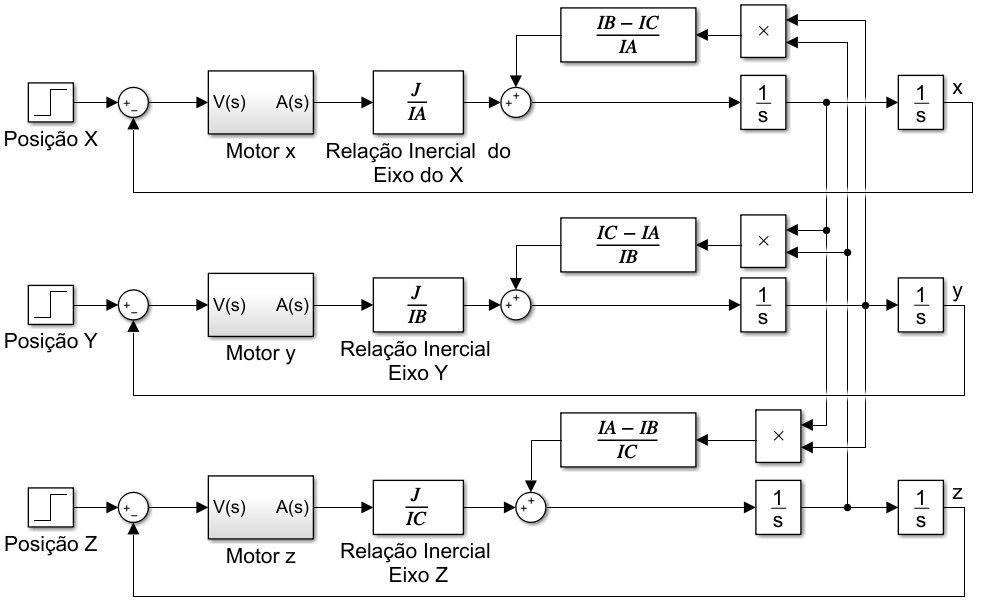
\includegraphics[scale=.6]{metodologia/img/simulink_modelo_completo_aberto}
  \end{center}
  \fonte{Elaborado pelo Autor.} 
  \label{fig:simulink_modelo_completo_aberto}
\end{figure}

Onde o bloco subsistema Motor x, y e z, é constituído pela função de transferência da equação \ref{eq:motor_accel}, que pode é inserida na ferramenta Matlab da seguinte forma:

\begin{figure}[H]
  \caption{Função de Transferência dos Motores}
  \begin{center}
      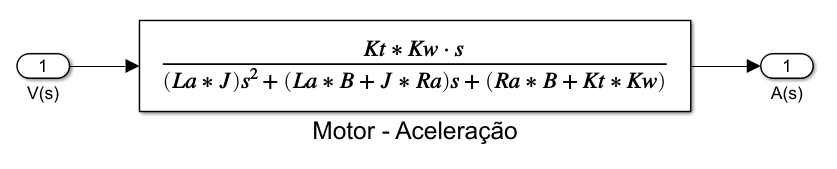
\includegraphics[scale=.45]{metodologia/img/modelo_satelite_motor}
  \end{center}
  \fonte{Elaborado pelo Autor.} 
  \label{fig:modelo_satelite_motor}
\end{figure}

Se fecharmos a malha em posição, usando um acelerômetro e usarmos um controlador PID, por consequência, conseguimos controlar a dinâmica do satélite em malha fechada. O diagrama de blocos com realimentação e com o controlador PID pode ser visto na figura \ref{fig:modelo_satelite_pid}. 

\begin{figure}[H]
  \caption{Modelo em malha fechada com um Controlador PID}
  \begin{center}
      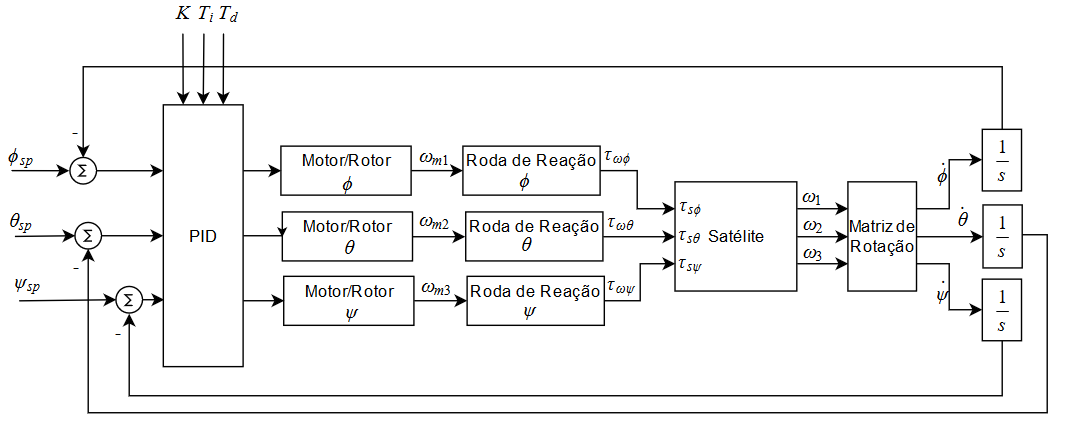
\includegraphics[scale=.6]{metodologia/img/modelo_satelite_pid}
  \end{center}
  \fonte{Elaborado pelo Autor.} 
  \label{fig:modelo_satelite_pid}
\end{figure}

Onde o bloco subsistema PID é constituído pelos seguintes blocos:

\begin{figure}[H]
  \caption{Digrama de Blocos do controlador PID com Anti-Windup}
  \begin{center}
      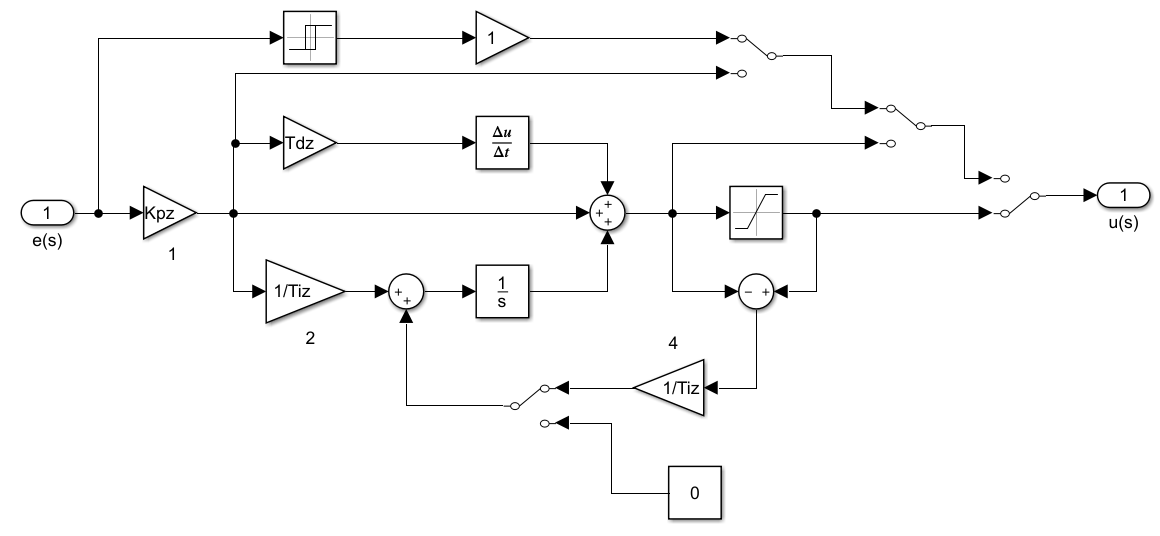
\includegraphics[scale=.45]{metodologia/img/matlab_pid_antiwindup}
  \end{center}
  \fonte{Elaborado pelo Autor.} 
  \label{fig:simulink_modelo_completo_aberto}
\end{figure}

Esse último diagrama é usado para o desenvolvimento do controle em software, onde os parâmetros do controlador são estimados pelos diferentes tipos de sintonia descritos na revisão bibliográfica. Na sequência, serão descritos os métodos que serão utilizados para implementar esse modelo em Python e embarcar isso na RPi.


%%%%%%%%%%%%%%%%%%%%%%%%%%%%%%%%%%%%%%%%%%%%%%%%%%%%%%%%%%%%%%%%%%%%%%

\section{Software}

Após a modelagem, devemos implementar o modelo e configurar todas as interfaces com os atuadores e sistema supervisório. A figura \ref{fig:comunicacao_projeto} descreve muito bem a forma que se dá a comunicação entre os periféricos, através da interface I2C para a RPi se comunicar com o acelerômetro/giroscópio, PWMs (Pulse Width Modulation - Modulação por Largura de Pulso) para a comunicação com os ESC e o protocolo SSH (Secure Shell) para a comunicação com o usuário.

\begin{figure}[H]
  \caption{Representação Geral do Sistema}
  \begin{center}
      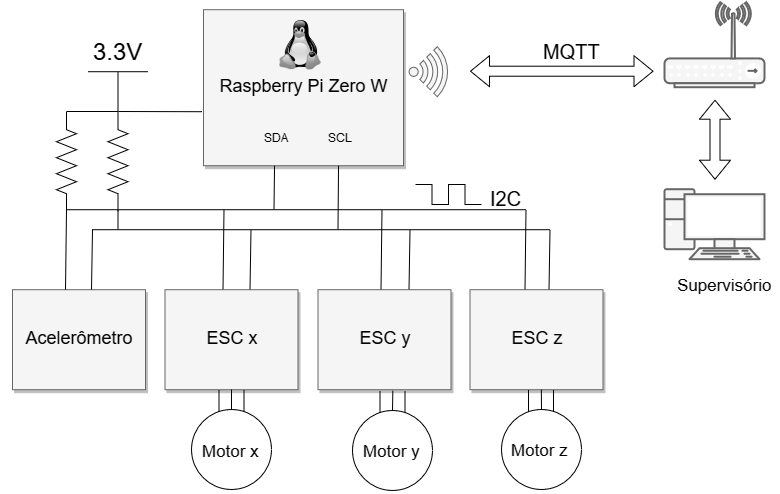
\includegraphics[scale=.65]{metodologia/img/comunicacao_projeto}
  \end{center}
  \fonte{Elaborado pelo Autor.} 
  \label{fig:comunicacao_projeto}
\end{figure}


Após modelada a topologia geral do sistema, é possível dividir a parte de software, onde é descita a implementação de cada etapa, começando com a implementação do controlador e da sua sintonia, que está na sequência.


%%%%%%%%%%%%%%%%%%%%%%%%%%%%%%%%%%%

\subsection{Implementação do Controlador PID e Métodos de Sintonia}

Nessa etapa ocorre a implementação usando a linguagem de programação Python, a qual, possui diversas bibliotecas de controle, interfaceamento e protocolos de comunicação. O desenvolvimento foi orientado para o menor tempo possível de atualização das entradas e saídas, pois, como é uma linguagem script sendo executada por um sistema operacional, algumas tarefas poderiam ser executadas em baixa prioridade, criando um comportamento não determinístico do período de amostragem. Uma solução para esse problema, foi a criação de uma interrupção via relógio que chama uma função de atualização das entradas e saídas, além do cálculo do PID e do filtro de Kalman. Na figura \ref{fig:software_model} podemos ver o fluxograma do scritp de controle.

\begin{figure}[H]
  \caption{Fluxograma do Software de Controle}
  \begin{center}
      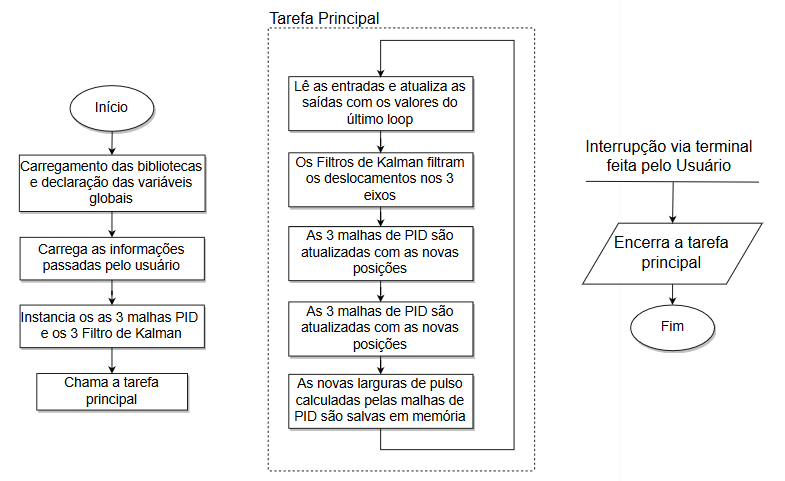
\includegraphics[scale=.95]{metodologia/img/software_model}
  \end{center}
  \fonte{Elaborado pelo Autor.} 
  \label{fig:software_model}
\end{figure}

Após o desenvolvimento das malhas de controle, e testes preliminares, ficou clara a grande influência dos sinais provenientes do giroscópio no resultado final, necessitando uma análise minuciosa para possibilitar a filtragem pelo filtro de Kalman e por consequência, controlar o simulador de satélites. Isso é abordado na sequência. 


%%%%%%%%%%%%%%%%%%%%%%%%%%%%%%%%%%%

\subsection{Análise dos Sinais e Filtragem}

Ao fazer os primeiros testes, ficou perceptível o bias (deslocamento em relação ao zero) e a gama de ruídos que compõem os sinais amostrados, isso pode ser visto na figura \ref{fig:bias_correction} (a), onde temos mais de 100.000 amostras nos três eixos. Já nas imagens \ref{fig:bias_correction} (b), (c) e (d), podemos ver o histograma dos mesmos sinais.

\begin{figure}[H]
  \caption{Características dos Sinais Amostrados pelo Giroscópio}
  %\begin{center}
      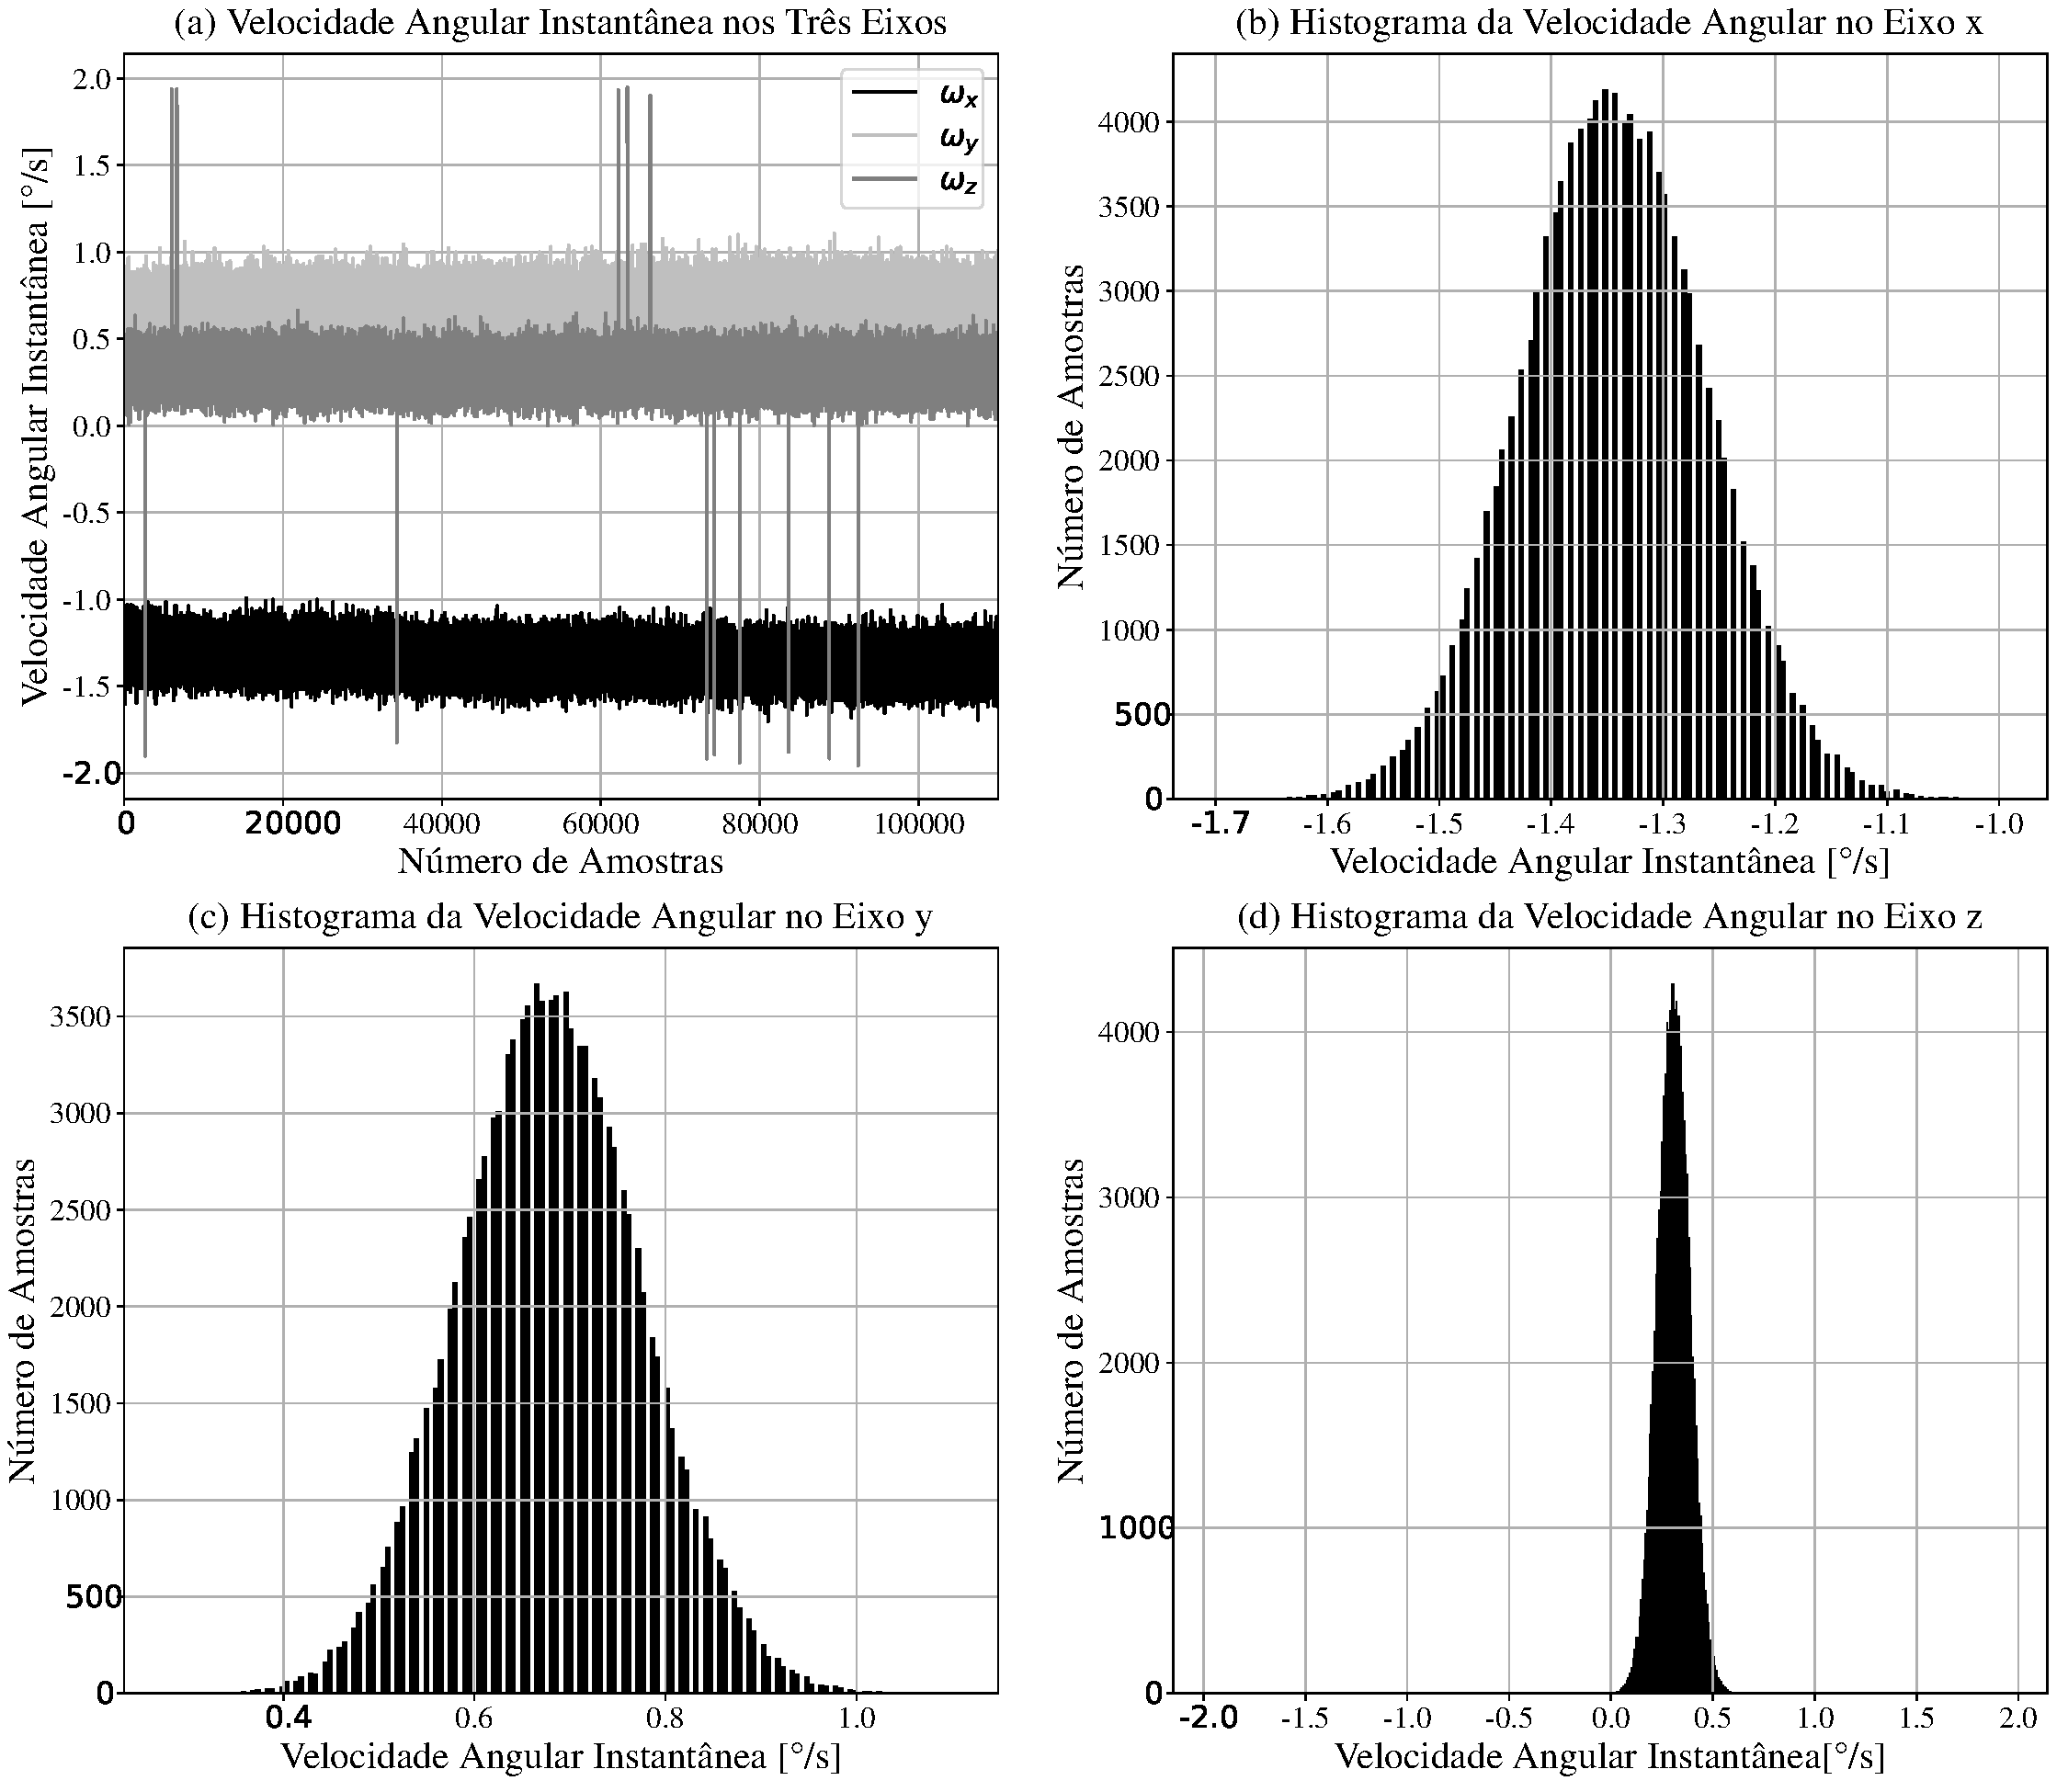
\includegraphics[scale=.4]{metodologia/img/bias_correction}
  %\end{center}
  \fonte{Elaborado pelo Autor.} 
  \label{fig:bias_correction}
\end{figure}

Como podemos ver, os três sinais possuem uma distribuição caraterística muito próxima de uma normal - mesmo que no eixo z exista ruídos espúrios maiores que nos demais eixos - o que valida o uso do Filtro de Kalman e a escolha da média aritmética das amostras como bias para as amostras do giroscópio. Os calores calculados pode ser vistos na tabela \ref{tab:bias_correction} 

\begin{table}[H]
  \caption{Correção do Bias do Giroscópio}
  \label{tab:bias_correction}
  \centering%
  \begin{minipage}{.42\textwidth}
    \begin{tabular*}{\textwidth}{cc}
      \hline
      {Eixo} & Velocidade Angular ($\omega [\SI{}{\degree\per\second}]$)\\ \hline
      \hline
      x  &  -1.3441 \\ 
      y  &  0.6797 \\
      z  &  0.3071 \\ \hline
    \end{tabular*}
    \fonte{Elaborado pelo Autor.} 
  \end{minipage}
\end{table}

Essa etapa corrigiu os problemas enfrentados, o próximo passo é sintonizar as malhas de controle, isso será descirto na sequência.


%%%%%%%%%%%%%%%%%%%%%%%%%%%%%%%%%%%

\subsection{Métodos de Sintonia}

O último passo da implementação do satélite, é a sintonia das malhas de controle, onde diferentes métodos foram utilizados para descobrir os parâmetros \textit{$K_p$}, \textit{$K_i$} e \textit{$K_d$}. Para isso, usamos um método clássico de sintonia, que é o de Ziegler-Nichols em malha fechada, o método do relé e por fim, o método automático usando redes neurais e regressão não-linear. Esses, serão descirtos na sequência. 


%%%%%%%%%%%%%%%%%%%%%%%%%%%%%%%%%%%

\subsubsection{Método de Ziegler-Nichols}

Como esse é um método heurístico, simplesmente precisamos captar as informações da resposta ao degrau em malha fechada para calcular os parâmetros do controlador. O processo é basicamente encontrar um ganho proporcional no qual a planta apresente um comportamento marginalmente estável, ou seja, possua uma oscilação sustentada na saída, onde conseguimos encontrar o valor do período de oscilação e o K crítico é o próprio ganho até a oscilação sustentada. Após a obtenção desses dois parâmetros, só calcularmos conforma a tabela \ref{tab:Ziegler-Nichols-freq}


%%%%%%%%%%%%%%%%%%%%%%%%%%%%%%%%%%%

\subsubsection{Método via RNA e Regressão Não-Linear}

Por fim, o método proposto pelo presente trabalho, onde diferentes conceitos foram empregados para a sintonia automática de controladores PID. Os dois usados, foram o de Redes Neurais e regressão não-linear robusta, de onde são extraídos os novo valores dos parâmetros. Na figura \ref{fig:neural_regression} podemos ver a topologia usada.

\begin{figure}[H]
  \caption{Diagrama de Blocos do Sintonizador e Otimizador}
  \begin{center}
      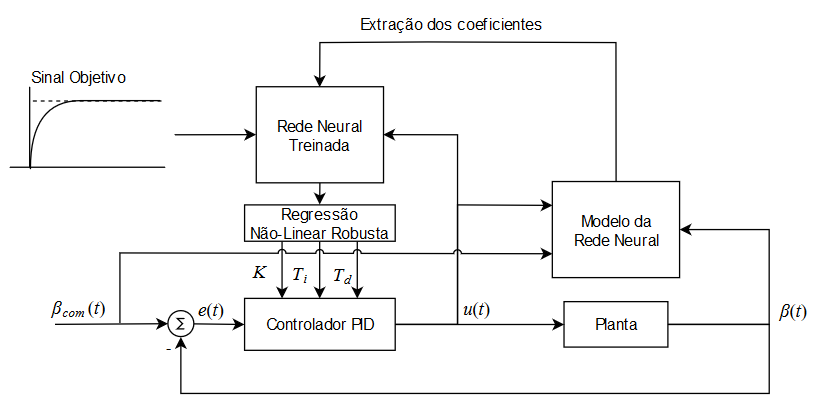
\includegraphics[scale=.65]{metodologia/img/neural_regression}
  \end{center}
  \fonte{Elaborado pelo Autor.} 
  \label{fig:neural_regression}
\end{figure}

O funcionamento dessa topologia é baseado na aprendizagem de máquina, onde uma rede neural aprende o comportamento do satélite, tendo como entradas a posição atual ($\beta$) , o valor de referência ($\beta_{com}$) e o sinal de controle, que nada mais é do que a largura de pulso entregue ao motor. Temos como saída da RNA, o sinal de controle, pois esse na prática, é um sinal modulado contendo a largura de pulso para o motor, onde a rede neural é mais assertiva devido ao comportamento não-linear, também característico de uma RNA. Após o treinamento da rede neural, ela é usada para se criar uma nova base de dados, onde ela recebe como parâmetros um sinal que é uma sugestão de resposta ao degrau (Sinal Objetivo) fornecida pelo usuário, ou ainda, uma representação do sistema em forma de um sistema de primeira ordem, pois esse, apresenta características melhores do que o sistema original. Basicamente, o objetivo de se fornecer esse sinal, é orientar a regressão não-linear ao ponto ótimo ou algo próximo a ele.

Por último, é feita e extração do parâmetros do controlador via regressão, onde o antigo sinal de controle é modulado através da variação dos coeficientes do controlador PID discreto até possuir a forma de onda do novo sinal, que foi gerado pela rede neural. Essa regressão é feita usando como função de minimização, o próprio controlador PID discreto, como pode ser visto na equação da sequência:

\begin{equation}\label{eq:motor_accel}
u(t) = K_c e(t) + \frac{K_c}{T_i}\sum_{n=0}^{N}{e(t)dt}-K_cT_d\frac{P[n]-P[n-1]}{dt}
\end{equation}

Onde essa equação é análoga as equações do controlador PID discreto, descritas no referencial teórico, onde dt é a diferença de tempo entre as amostras, P é a variável de interesse, e(t) é o erro instantâneo. A partir dessa equação, podemos implementar uma função de minimização, que está no script em Python da sequência:

\begin{lstlisting}[caption={Pseudocódigo I: Minimização da Função do Controlador}]
funcao(x, n, y_original) :
    erro = referencia - dados_objetivo[n]
    se (n>0) :
        soma_erro += erro
        derivada =  (dados_objetivo[n] -  dados_objetivo[n-1]/dt
        saida_controlador = Kp * erro + (Kp/Ti)*soma_erro*dt - Kp*Td*derivada
    se nao :
        saida_controlador = 0
    n += 1
    retorna u - y_original
\end{lstlisting}

Onde $x[0]$ é \textit{$K_p$}, $x[1]$ é \textit{$T_i$}, $x[2]$ é \textit{$T_d$}, \textit{soma\_erro} é o somatório do erro, \textit{derivada} é a derivada da variável de interesse, \textit{dado\_teste} é o dado proveniente da RNA treinada, \textit{n\_t} é o vetor com o número das amostras, \textit{u} é a saída do controlador, \textit{y} é saída do controlador não sintonizado, \textit{n} é o indexador de cada interação. Com isso, conseguimos extrair os novos parâmetros do controlador.
